% !TeX root=../main.tex

\section{Introduction}
\label{introduction}
Trace alignment is a well-known technique in conformance checking \cite{DBLP:conf/edoc/AdriansyahDA11} providing both a numerical assessment of the degree of conformance of a log trace with respect to a model, as well as a repair strategy if such trace does not conforms to the given model. At the time of the writing, 
%
%In the existing literature on conformance checking, a common approach is based on trace alignment \cite{DBLP:conf/edoc/AdriansyahDA11}. However, this approach uses crisp process models as reference models. On the other hand, recently, 
existing probabilistic conformance checking approaches %are gaining momentum
 %, but
provide a numerical quantification of the degree of conformance
%the existing approaches are used to check the degree of conformance 
of a trace log with respect to a stochastic process model \cite{DBLP:journals/tosem/PolyvyanyySWCM20}
by either assessing the distribution discrepancies \cite{DBLP:conf/bpm/LeemansSA19}, or by exploiting entropy-based measures \cite{DBLP:conf/icpm/PolyvyanyyK19}. As these strategies are not based on trace alignments, these cannot be directly exploited to repair the given log trace with one of the traces generated by stochastic process model. As traces generated by stochastic process models, namely  stochastic Workflow nets, are associated to a probability representing its likelihood within the model, the trace alignment should also take into account such measure as likelier traces should be preferred.
%instead of finding trace alignments.
In this paper, we provide for the first time a conformance checking approach based on trace alignments using a stochastic reference
model.
%Conceptually, this requires to handle the two possibly contrasting forces of the cost of the alignment on the one hand and the
%likelihood of the model trace with respect to which the alignment is computed. We consider the important tradeoff between both
%aspects.

%Balancing between the likelihood of the model trace with respect to which we are computing the alignment and the cost of the alignment (if the cost of the alignment is too high even if the model trace is very likely applying too many changes in the original trace is in turn not very likely).

\begin{figure}[!t]
	\centering
	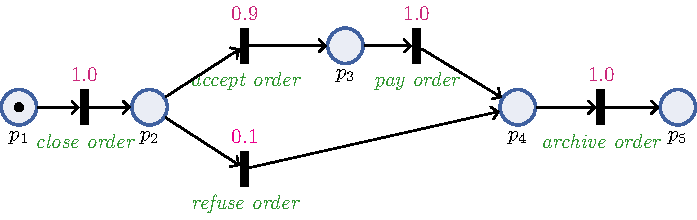
\includegraphics[width=.6\textwidth]{images/petri_tut.pdf}
	\caption{Stochastic Workflow Network modeling our use-case scenario.}\label{fig:petri_tut}
\end{figure}
An alignment of a trace with a stochastic net could be represented by the model trace maximizing the combined provision of minimum trace alignment cost and maximum model trace probability. With reference to Figure~\ref{fig:petri_tut}, an user might be interested to align the log trace $\braket{\textsf{close order},\,\textsf{archive order}}$ with one of the two model traces, i.e., $\langle\textsf{close order},\,\textsf{accept order},\,\textsf{pay order},\,\textsf{archive order}\rangle$ or $\langle\textsf{close order},\,\textsf{refuse order},\,\textsf{archive} \textsf{order}\rangle$. While the  latter trace provides the least alignment cost though the model trace has the minimum probability ($0.1$), the former gives a slightly greater alignment cost while providing the maximum probability ($0.9$). Given that, depending on the context, users might prefer either the former or the latter alignment, a selection of the best $k$ alignments among all the distinct model traces empowers the users to find their own trade-off between alignment cost and model trace probability.
%However, in some cases, the user could prefer to identify an alignment with a lower cost even if based on a less probable model trace, while, in other cases, the user could favor a model trace with a higher probability at the expense of a higher alignment cost. Therefore, to provide users with an instrument that allows them to find their own trade-off between alignment cost and model trace probability, we need to return the best $k$ alignments among all the distinct model traces. 
To do this, we frame the probabilistic trace alignment problem into the the well-known $k$-Nearest Neighbors ($k$NN) problem \cite{Altman} that refers to finding the $k$ nearest data points to a \textit{query} $x$ from a set $\mathcal{X}$ of \textit{data points} via a distance function defined over $\mathcal{X}\cup\{x\}$.


%Since when aligning an event log with a stochastic net distinct model traces have different probabilities, the retrieval of the best model trace maximizing the combined provision of minimum trace alignment cost and maximum model trace probability might not suffice. In some cases, indeed, the user could prefer to identify an alignment with a lower cost even if based on a less probable model trace, while, in other cases, the user could favor a model trace with a higher probability at the expense of a higher alignment cost. We consider, therefore, the important tradeoff between both aspects.
%Therefore, in this paper, we propose trace alignment approaches that return the best

We introduce two ranking strategies. The first one is based on a brute force approach that reuses existing trace aligners such as \cite{DBLP:conf/edoc/AdriansyahDA11,LeoniM17}, where the (optimal) ranking of the top-k alignments is obtained by computing the Levensthein distance between the trace to be aligned and all the model traces and by multiplying each of these distance by the probability of the corresponding model trace. However, even if this approach returns the best trace alignment ranking for a query trace, the alignments must be computed a-new for all the possible traces to be aligned. For models generating a large number of model traces, this would clearly become unfeasible. Therefore, we propose a second strategy that produces an approximate ranking where $x$ and $\mathcal{X}$ are represented as numerical vectors via an embedding $\phi$. {Then, by exploiting ad-hoc data structures,
%such as Vp-Trees \cite{Fu2000}, Kd-Trees \cite{Maneewongvatana99}, and M-Trees \cite{Ciaccia},
we can retrieve the neighborhood of $x$ in $\mathcal{X}$ of size $k$  by pre-ordering (\textit{indexing}) $\mathcal{X}$  via a distance between the numerical vectors obtained using $\phi$. Thus, we do not need to analyze the entire space, but just start the search from the top-$1$ alignment. If the embeddings $\phi$ for $\mathcal{X}$ are independent of the query of choice $x$, this would not require to constantly recompute the numeric vector representation for $\mathcal{X}$.
%	

%%%%% Proposed part as the last part of the introduction:
%\texttt{\color{red}[TODO]}
%\todo{this is too specific for an introduction; in particular, too many details on how the experiments are done.}
We implemented both strategies\footnote{\url{https://github.com/jackbergus/approxProbTraceAlign}} and perform experiments using a real life event log coming from an hospital system to empirically evaluate the properties of our proposed  strategy. Specifically, we (i) evaluate the correlation between the approximate rankings (using different ways for computing the embeddings) and the optimal ranking, and (ii)~compare the computation time for the exact trace alignment approach against the embedding-based approach. We show that the approximate ranking strategy exploiting a specific data structure (KD-Trees) provides the best trade-off between approximation and execution time, while being more efficient than both the exact ranking and the same approximate ranking with a different data structure (VP-Trees).


